%!TEX root = ../report.tex
\section{Results} % (fold)
\label{sec:results}
	\subsection{Implementation} % (fold)
	\label{sub:implementation}
	The ANNGA player consists of two parts: (1) the ANN player and (2) the genetic algorithm. 
	The ANN player has been implemented using the \emph{Encog} Libraries \cite{encog} that makes uses of multi threading and even GPU to compute some operations.
	This library is used to create the ANN and train it based on the situations and the chromosome.

	The GA has been implemented making use of the multi threading capabilities of Java. 
	Due to the machine used has an 8 threaded processor, in each generation 8 tournaments are played in parallel.
	This makes the ANNGA improves 8 times faster compared with a single threaded GA.
	Despite the low number of threads makes the population really small, the high speed computation of the CPU makes the GA give good results.

	\subsubsection{Computation time} % (fold)
	\label{ssub:computation_time}
		The machine has a processor Intel® Core™ i7-4702HQ CPU @ 2.20GHz 8x and 16 GB of RAM.
		When running, the computer uses the 100\% of each thread and around 1.2 GB of RAM.
		In each thread, 1000 games last around 600 ms which means that, if 8 threads are used, 8000 games are done in the same time. 	
		The number of generations per second depends entirely on the number of games in a tournament, then this is determinant to find a good solution.
	% subsubsection computation_time (end)

	\subsection{Luck factor analysis} % (fold)
	\label{sub:luck_factor_analysis}
	Trying optimize the computation time, an study of the luck factor is made. 
	The tournaments are made to reduce the luck component and determine the real skill of the player.
	Despite the by default 1000 games are played in a tournament, the luck factor have been analyzed.
	For this purpose, four ANN players with the same chromosome are made to play a defined number of games.
	When finished, the mean of points is obtained taking that value as what defines the skill of the player.
	Then, an sample of games is taken and its mean is calculated and compared with the global mean.
	This means are used create an sample standard deviation analysis and the result is that the pseudo random number generation is \emph{patterned} (Fig. \ref{fig:luck_evolution}).
		\begin{figure}[!ht]
			\centering
			\begin{subfigure}{.33\textwidth}
			  \centering
			  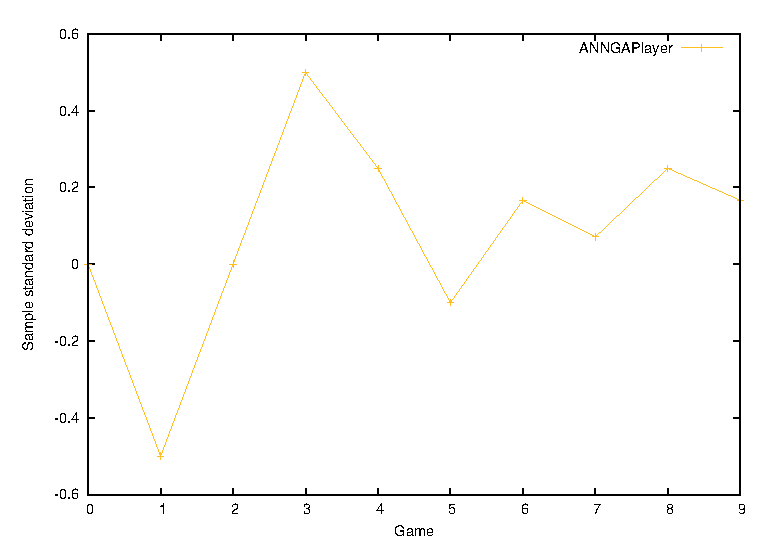
\includegraphics[width=\textwidth]{figures/luck_evolution_10}
			  \caption{Sample standard deviation for 10 games}
			  \label{fig:luck_evolition_10}
			\end{subfigure}%
			\begin{subfigure}{.33\textwidth}
			  \centering
			  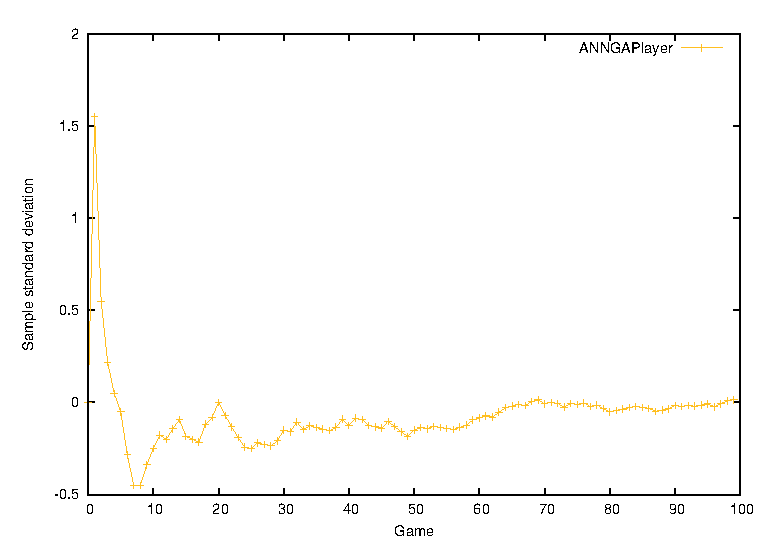
\includegraphics[width=\textwidth]{figures/luck_evolution_100}
			  \caption{Sample standard deviation for 100 games}
			  \label{fig:luck_evolition_100}
			\end{subfigure}%
			\begin{subfigure}{.33\textwidth}
			  \centering
			  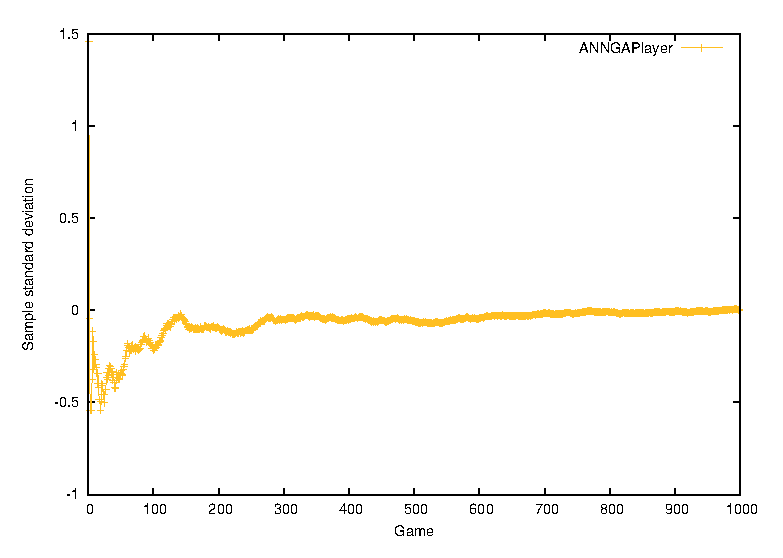
\includegraphics[width=\textwidth]{figures/luck_evolution_1000}
			  \caption{Sample standard deviation for 1000 games}
			  \label{fig:luck_evolition_1000}
			\end{subfigure}%
			\caption{Analysis of the luck component to determine how many games to play in a tournament}
			\label{fig:luck_evolution}
		\end{figure}

	A stable result is considered when the sample standard deviation is in $\pm 0.2$.
	When the games in a tournament are more than 10, for example 100 (Fig. \ref{fig:luck_evolition_100}), a stable result is found around the 30\% of the experiment, which would lead to think that 30 games is enough to eliminate the luck component.
	However, when the same experiment is carried out for 1000 games, the stabilization comes with 300, and no 30, again around 30\%.
	This experiment has been repeated with different samples and the conclusion is than above 10 games, the uncertainty becomes acceptable always.
	This could be due to the way of generate random numbers that Java has, so at some point the random numbers stops being random and generates a pattern.
	% subsection luck_factor_analysis (end)

	\subsection{LUDO player comparison} % (fold)
	\label{sub:ludo_player_comparison}
	To analyze the skill of the ANNGA player, is compared with other players already implemented in the code and others from other students.
	This section starts analyzing the fitness function when playing against SemiSmarts players. 
	Then an analysis for the best chromosome of the evolution compared (named \emph{the legend}) and the best one from the last generation is made.
	Finally, a group tournament is made with the players of some classmates.
	For this tournament one chromosome has to be chosen to play.
		\subsubsection{ANN evolution} % (fold)
		\label{ssub:ann_evolution}
		Based on the luck factor analysis [\ref{sub:luck_factor_analysis}], instead of the 1000 games given by default, the tournaments are made with 300. 
		This suppose an improvement of 66\% in time computation with the same results, which improves the GA.
		As the selection in the GA can be made based on \emph{won games} or \emph{accumulated points}, the total points also varies.
		However, the results are given in a percentage of the points given to make it independent of the number of games.
		The fitness function shows the evolution of the population in each generation. \\

		Two studies have been carried out (Fig \ref{fig:fitness_won} and Fig \ref{fig:fitness_distributed_points}) for 500 generations, 300 games tournament, being the ANNGA player the first, with a uniform crossover and $\pm 0.2$ in mutation with a random mask. \\

			\begin{figure}[!ht]
				\centering
				\begin{subfigure}{.5\textwidth}
				  \centering
				  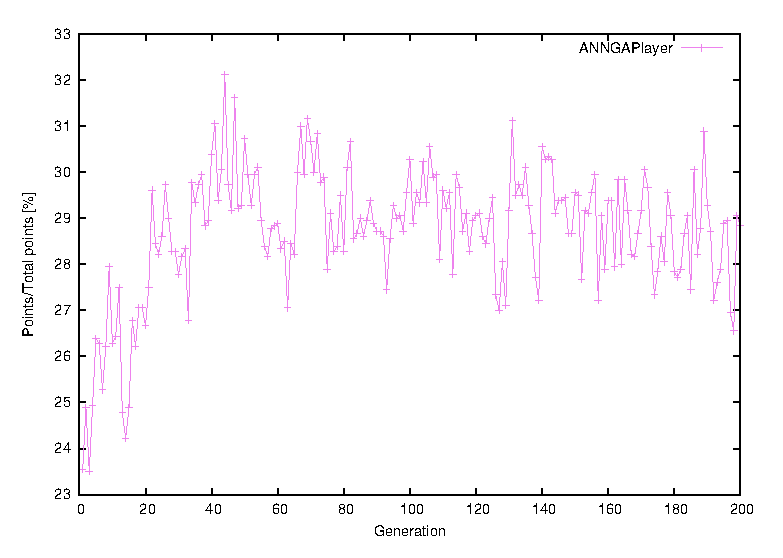
\includegraphics[width=\textwidth]{figures/fitness_won}
				  \caption{Fitness function when selecting only with won games}
				  \label{fig:fitness_won}
				\end{subfigure}%
				\begin{subfigure}{.5\textwidth}
				  \centering
				  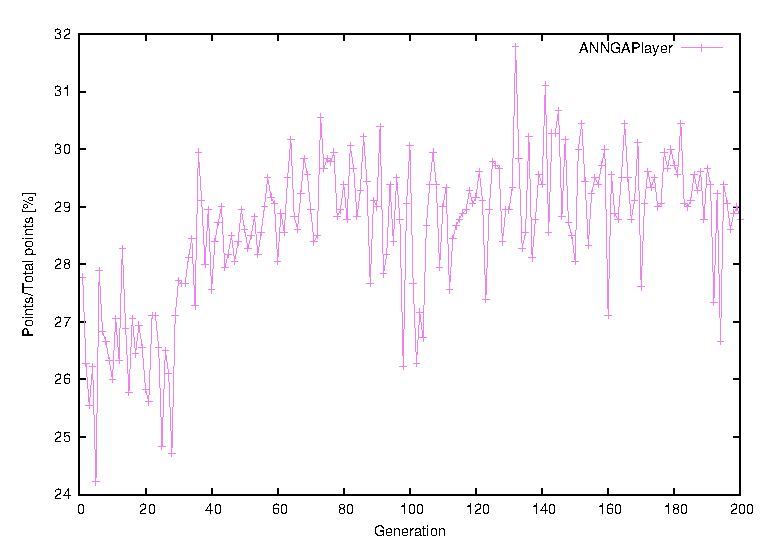
\includegraphics[width=\textwidth]{figures/fitness_distributed_points}
				  \caption{Fitness function when selecting with distributed points}
				  \label{fig:fitness_distributed_points}
				\end{subfigure}
			\end{figure}
		In both plots the improvement stabilizes around 29\% of the possible points in the generation 40.
		However, the worst generation gets 24\% of the points which means that wins almost all the games from an early stage.
		This with the fact that the highest success rate is not over 31\% makes the fitness function quite small in improvement terms.
		No significant differences are found between selecting with the won games and the distributed points.

		% subsubsection ann_evolution (end)

		\subsubsection{The legend chromosome} % (fold)
		\label{subs:the_legend_chromosome}
		Due to the LUDO game is a game of chances, perhaps the last generation is not the one with most points.
		For this reason the best chromosome during the evolution is stored and compared with the best one in the last generation.
		This chromosome is called \emph{the legend}.
		The comparison is only made playing a tournament being both ANNGA players the first ones and playing 10000 games against three SemiSmarts (Fig \ref{fig:the_legend_comparison}). \\
		
			\begin{figure}[!ht]
				\centering
				\begin{subfigure}{.5\textwidth}
				  \centering
				  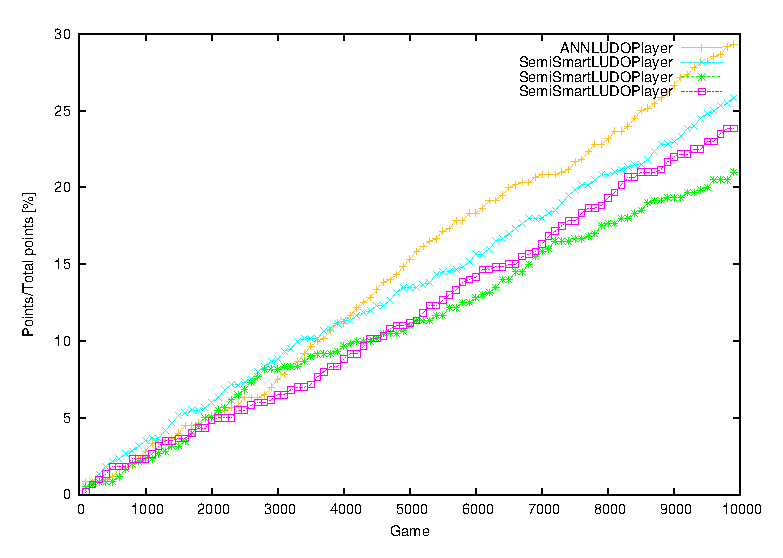
\includegraphics[width=\textwidth]{figures/the_legend_last_generation}

				\end{subfigure}%
				\begin{subfigure}{.5\textwidth}
				  \centering
				  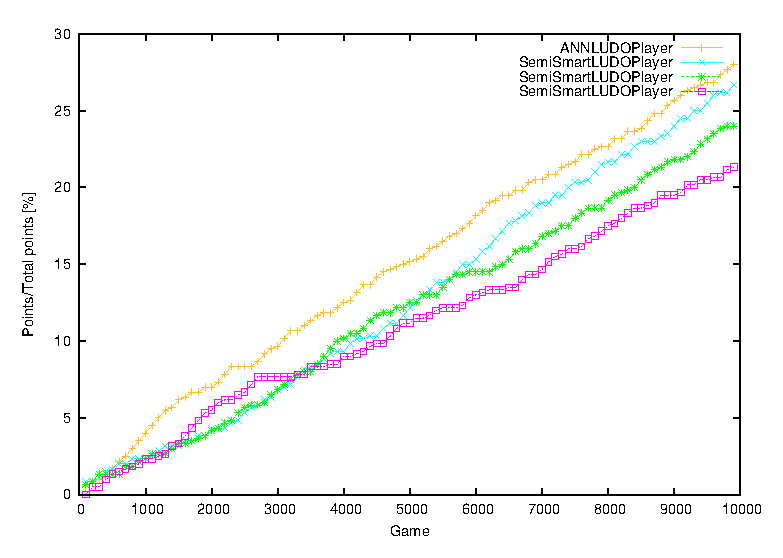
\includegraphics[width=\textwidth]{figures/the_legend_the_legend}
				\end{subfigure}
				\caption{Comparison of the results between \emph{the legend} (Right) and the best chromosome of the last generation (Left)}
				\label{fig:the_legend_comparison}
			\end{figure}
		The results shows how last generation perform slightly better, but enough to carry out the rest of the experiments with the last generation.

		\subsubsection{Group tournament} % (fold)
		\label{ssub:group_tournament}
		A tournament against the AIs from other students has been carried out. The tournament has been made with an ANNGA player, a SemiSmart, a Q-learner with GA from Carlos Moro \cite{carlos} and a NN player from Ignacio Torroba \cite{nacho}.
		\begin{itemize}
			\item \emph{The Reinforcement Learning with GA player}. 
			This player implements a Q-learning algorithm with 9 actions and 7 states. 
			The rewards are changed with a GA, as in the ANNGA player, and then adjusted with a learning rate and a discount factor. 
			This approach is potentially better than the ANNGA due to it contain more information than the ANNGA chromosome.
			\item \emph{ANN Player}. This player is as the ANN player explained in this paper with two differences: (1) the internal structure is different having 25 neurons in the hidden layer and (2) the situation of the game is analyzed global, not for each brick. 
			This leads to a global analysis that contains perhaps more information about the game compared with the ANNGA player.
			The ANN learns from a trainer agent that is based on a predefined actions.
		\end{itemize}

		The test was made during 10000 games and the chromosome chosen for the ANNGA was: (0.45, 1.00, 0.00, 0.63, 0.48, 0.10, 0.00, 0.94, 0.74, 0.66, 0.93, 0.15, 0.00, 0.95, 0.40, 0.11, 0.30).
		This chromosome was evolved during for 500 generation, 300 games tournament, being the ANNGA player the first, with a uniform crossover and $\pm 0.2$ in mutation with a random mask.
		Two tournaments were made, one counting the games won and other with the distributed points.
			\begin{figure}[!ht]
				\centering
				\begin{subfigure}{.5\textwidth}
				  \centering
				  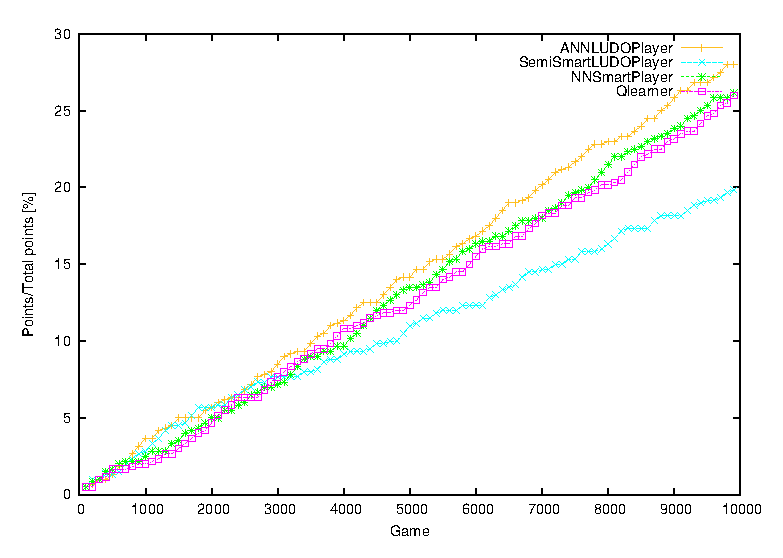
\includegraphics[width=\textwidth]{figures/competition_points}
				  \caption{Competition with distributed points}
				  \label{fig:competition_points}
				\end{subfigure}%
				\begin{subfigure}{.5\textwidth}
				  \centering
				  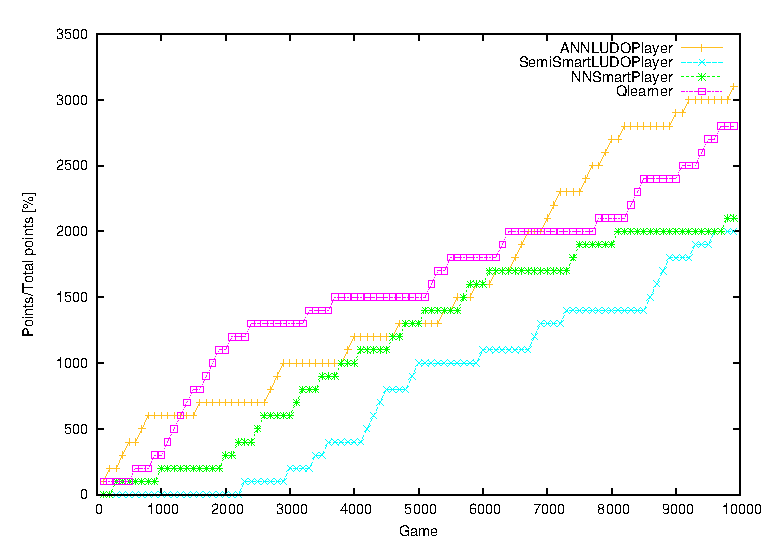
\includegraphics[width=\textwidth]{figures/competition_won}
				  \caption{Competition only with won games}
				  \label{fig:competition_won}
				\end{subfigure}
				\caption{Competition for 10000 games comparing won games and distributed points. ANNGA vs NN vs Q-learner vs SemiSmart}
				\label{fig:competition}
			\end{figure}

		The results (Fig \ref{fig:competition}) shows how the ANNGA player performs better in both situations.
		% subsubsection group_tournament (end)

	% subsection ludo_player_comparison (end)


% section results (end)